\documentclass{article}

\PassOptionsToPackage{numbers}{natbib}
\usepackage[final]{neurips_2023} % provided style file

\usepackage[utf8]{inputenc} % allow utf-8 input
\usepackage[T1]{fontenc}    % use 8-bit T1 fonts
\usepackage{hyperref}       % hyperlinks
\usepackage{url}            % simple URL typesetting
\usepackage{booktabs}       % professional-quality tables
\usepackage{amsfonts}       % blackboard math symbols
\usepackage{nicefrac}       % compact symbols for 1/2, etc.
\usepackage{microtype}      % microtypography

\usepackage{tabularx} % For tables with specified width
\usepackage{hyperref} % For hyperlinks
\usepackage{booktabs} % For better table lines
\usepackage{graphicx} % For including images
\usepackage{subcaption} % For subfigures

\usepackage{amsfonts}

\bibliographystyle{unsrtnat}
\usepackage{float}

\title{Predicting Cell Types in Non-Human Single Cell RNA Sequencing Data}

\author{
  Sean Connelly \\
  % examples of more authors
  \And
  Ryan Videgar-Laird \\
  \AND
  Stephanie Ting \\
}

\begin{document}

\maketitle

\section{Introduction}

The biology that underlies disease is heterogeneous, with multiple cell types and pathways within those cell types that contribute to the development of disease. All cells have DNA, the genetic code, that is transcribed into messenger RNA (mRNA), called gene expression. After these genes are expressed, the mRNA is then translated into proteins, which go on to perform different functions. mRNA can be expressed at different levels, depending on which proteins are needed by the given cell type. These different levels of mRNA expression can characterize cells and allow further analysis of their contribution to disease biology \cite{segundo-valIntroductionGeneExpression2016}.
 
 The mRNA produced can be quantified at the cellular level, called single cell RNA sequencing (scRNAseq), to obtain a ‘fingerprint’ of different cell types and can be compared between normal or disease conditions to find how these cell types change. scRNAseq data is processed into a gene expression matrix, which has dimensions of m cells x n genes. After performing quality control steps, normalizing and scaling this gene expression matrix, this matrix undergoes dimensionality reduction to compress this dataset that contains many features (genes) to see how these cells relate to one another. The patterns of how cells vary compared to one another can be clustered using any algorithm of one’s choosing. The resulting clusters represent certain types of cells that need to be characterized and classified \cite{aljanahiIntroductionAnalysisSingleCell2018}.

Classifying single cells has mainly focused on utilizing three categories of techniques. The first class of techniques annotate these clusters through comparing the differential expression (greater number of counts) of the genes in a given cluster with every other cluster through statistical tests, like the Wilcoxon rank sum test. These differentially abundant genes in each cluster can be compared to experimentally validated genes that characterize cell types to identify the label for that cluster. The second class of techniques correlates the newly generated dataset with a reference dataset to annotate cell clusters. This reference dataset can be other single cell RNA sequencing data or bulk RNA sequencing of specific cell types individually or over a time series. Lastly, the third class of techniques uses supervised learning, which utilizes previously generated data to train a model to classify cell types. Many recommended pipelines utilize standard methods, such as logistic regression, support vector machine or random forest models \cite{heumosBestPracticesSinglecell2023}.

Many of these tasks have been focused on human data, where there has been much focus on diseases, like different forms of cancer, that affect many people domestically, but not much focus on diseases that have broad impacts globally. One such disease is malaria, a parasitic infection that resulted in 247 million cases in 2021 and causes a large burden of morbidity and mortality globally \cite{organizationWorldMalariaReport2022}. Malaria has a complex life cycle, which starts in the mosquito vector to result in infection of a human host. When individuals are sick with malaria, the parasite replicates in the blood cells and causes these blood cells to lyse when the parasite replicates. These replication stages have unique gene expression patterns and single cell RNA sequencing provides a key benefit to further understand how these genes change per cell stage. These same concepts can be applied to other neglected diseases and hosts. From looking at developmental trajectories in zebrafish \cite{farrellSinglecellReconstructionDevelopmental2018} to COVID-19 response in non-human primates \cite{speranzaSinglecellRNASequencing2021} to single cell RNA sequencing of other parasitic diseases \cite{briggsSinglecellTranscriptomicAnalysis2021, wendtSinglecellRNAseqAtlas2020, rezvaniComparativeSinglecellTranscriptional2022}, we would like to build a powerful, simple and efficient model that can classify cell types on this source of data.

\subsection{Related Work}

Two previous studies have introduced methods that successfully use attention based models to predict cell type in scRNAseq. The first one, TOSICA, uses a three part approach of cell embedding, multi-head self attention, and then cell type classification \cite{chenTransformerOneStop2023}. TOSICA is highly accurate for both mouse and human data. This model, however, relies on curated expert knowledge in the cell embedding stage to provide pathway information critical to identifying cell types. The second model, scBERT, uses an adaptation of BERT, a natural language processing model on scRNAseq where the transformer architecture is replaced with a performer in order to better handle larger scale input data \cite{yangScBERTLargescalePretrained2022}. This model is trained with data from millions of cells from a variety of different biological contexts. scBERT not only predicts cell type with very high accuracy, it also has interpretability in that the prediction rediscovers known biomarker genes of each cell type. However, scBERT does require an immense amount of training data and has only been tested on human data. It is also a complex model that is computationally intensive. 

Our approach is to use these methods as a foundation to build a simpler model that is less computationally expensive and works on non-human, non-mouse datasets. Our model will also not rely on manual curation of knowledge, which is often inconsistently annotated and formatted.

\section{Methods}

Anndata \cite{virshupAnndataAnnotatedData2021} and Scanpy \cite{wolfSCANPYLargescaleSinglecell2018} were used to create efficient data objects and  follow best practices for scRNA-seq analysis. This includes: filtering out cells that express less than 100-200 genes, removing genes that are observed in less than 3 cells, and applying a shifted logarithm transformation. These quality control (QC) steps help reduce noise from experimental prep from sources such as low quality cells and environmental contamination, and stabilize variance across cells \cite{heumosBestPracticesSinglecell2023}. 

Let \(y\) represent total gene counts for a given cell, and \(s_c\) represent the size factor for that cell. Counts are then shifted by:

\begin{displaymath}
% \label{eq:log_trans}
f(y) = log\left(\frac{y}{s_c} + y_0 \right)
\end{displaymath}

The size factor for a given cell designed to account for variation in cell size (larger cells typically contain more genetic transcripts) and sampling effects. Let \(L\) represent the median raw count depth across all cells. Then \(s_c\) is calculated across all genes, \(g\), per cell: 

\begin{displaymath}
% \label{eq:s_c}
s_c = \frac{\sum_g y_{gc}}{L}
\end{displaymath}

More information on developing a transformer model in Future Work section. 

\section{Preliminary Results}

\subsection{Traditional Methods}

We began with a scRNAseq dataset (\emph{P. falciparum}) from the Malaria Cell Atlas \cite{howickMalariaCellAtlas2019} to test out various supervised classification models. We began with this dataset as it is small and therefore easy to use on local machines while gaining familiarity with the methods. In addition, standard techniques have been shown to perform well on it \cite{shuklaSupervisedLearningPlasmodium2023}, so it serves as a good baseline for later comparisons. 

Principal Component Analysis was performed to visualize how the given cells vary compared to one another. The cells are well stratified by developmental stage (Figure \ref{fig:pfal_pca_true}). To test the performance of two classic models for classification tasks, we used logistic regression (LR) and support vector machines (SVM), implemented through Scikit-learn \cite{pedregosaScikitlearnMachineLearning2011}. To incorporate more graph based information in our model, we used an implementation of a graph convolutional network in the Spektral package \cite{grattarolaGraphNeuralNetworks2020}, based on the work of Kipf and Welling \cite{kipfSemiSupervisedClassificationGraph2017}. The data was split into a 70\% training and 30\% test split. The input to the model was the filtered and normalized gene expression matrix along with the cell type labels. For each model, we labeled the cells in the PCA as correct (blue) or incorrect (orange). Incorrectly predicted cells were spread throughout the PCA and did not concentrate within a certain cell type across all models (Figure \ref{fig:pfal_pca_pred}). 

\begin{figure}[H]
	\centering
  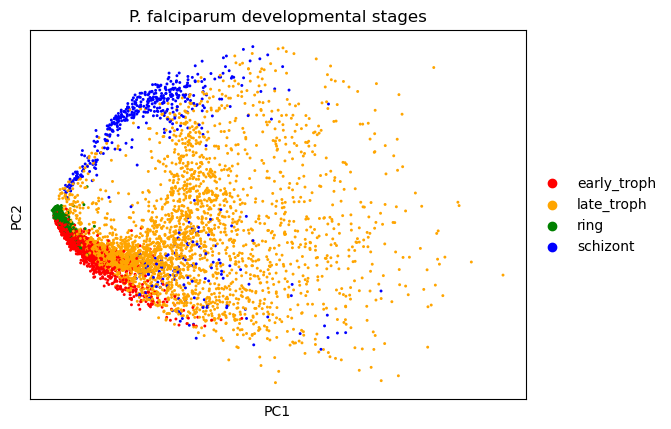
\includegraphics[width=0.8\textwidth]{figures/pca_Pf.png}
  \caption{Principal components analysis of \textit{P. falciparum} single cell RNA sequencing data, colored by lifecycle stage.}
  \label{fig:pfal_pca_true}
\end{figure}

\begin{figure}[!h]
  \centering
  \begin{subfigure}[b]{0.3\textwidth}
      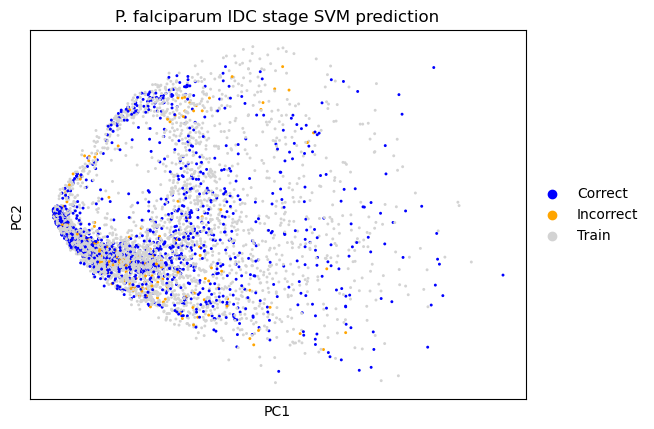
\includegraphics[width=\textwidth]{figures/pca_Pf_prediction_SVM.png}
      \caption{PCA of predictions from SVM model.}
      % \label{fig:sub1}
  \end{subfigure}
  \hfill
  \begin{subfigure}[b]{0.3\textwidth}
      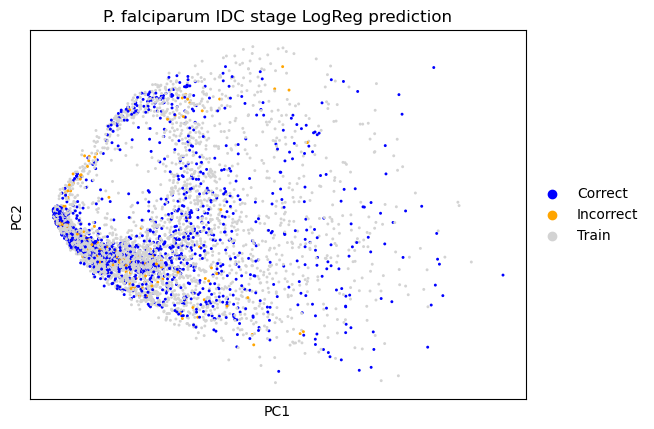
\includegraphics[width=\textwidth]{figures/pca_Pf_prediction_LogReg.png}
      \caption{PCA of predictions from logistic regression model.}
      % \label{fig:sub2}
  \end{subfigure}
  \hfill
  \begin{subfigure}[b]{0.3\textwidth}
      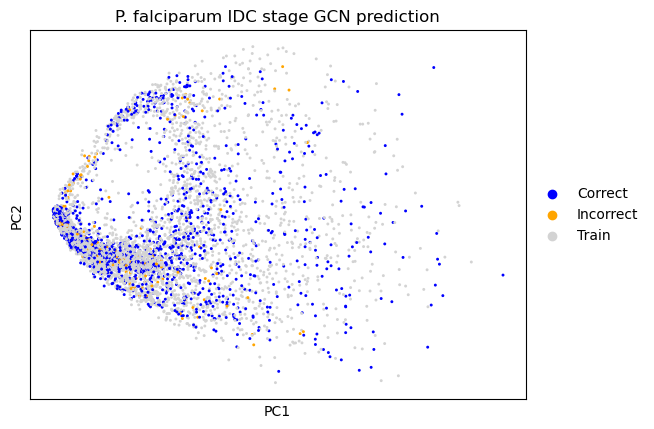
\includegraphics[width=\textwidth]{figures/pca_Pf_prediction_GCN.png}
      \caption{PCA of predictions from graph convolutional network model.}
      % \label{fig:sub3}
  \end{subfigure}
  
  \caption{Model performance visualized on PCA plots.}
  \label{fig:pfal_pca_pred}
\end{figure}


In addition, the F1 score was calculated per cell type. All cell type prediction methods were above 80\% and very similar among the three models (Figure \ref{fig:pfal_pred_f1}).

\begin{figure}[H]
  \centering
  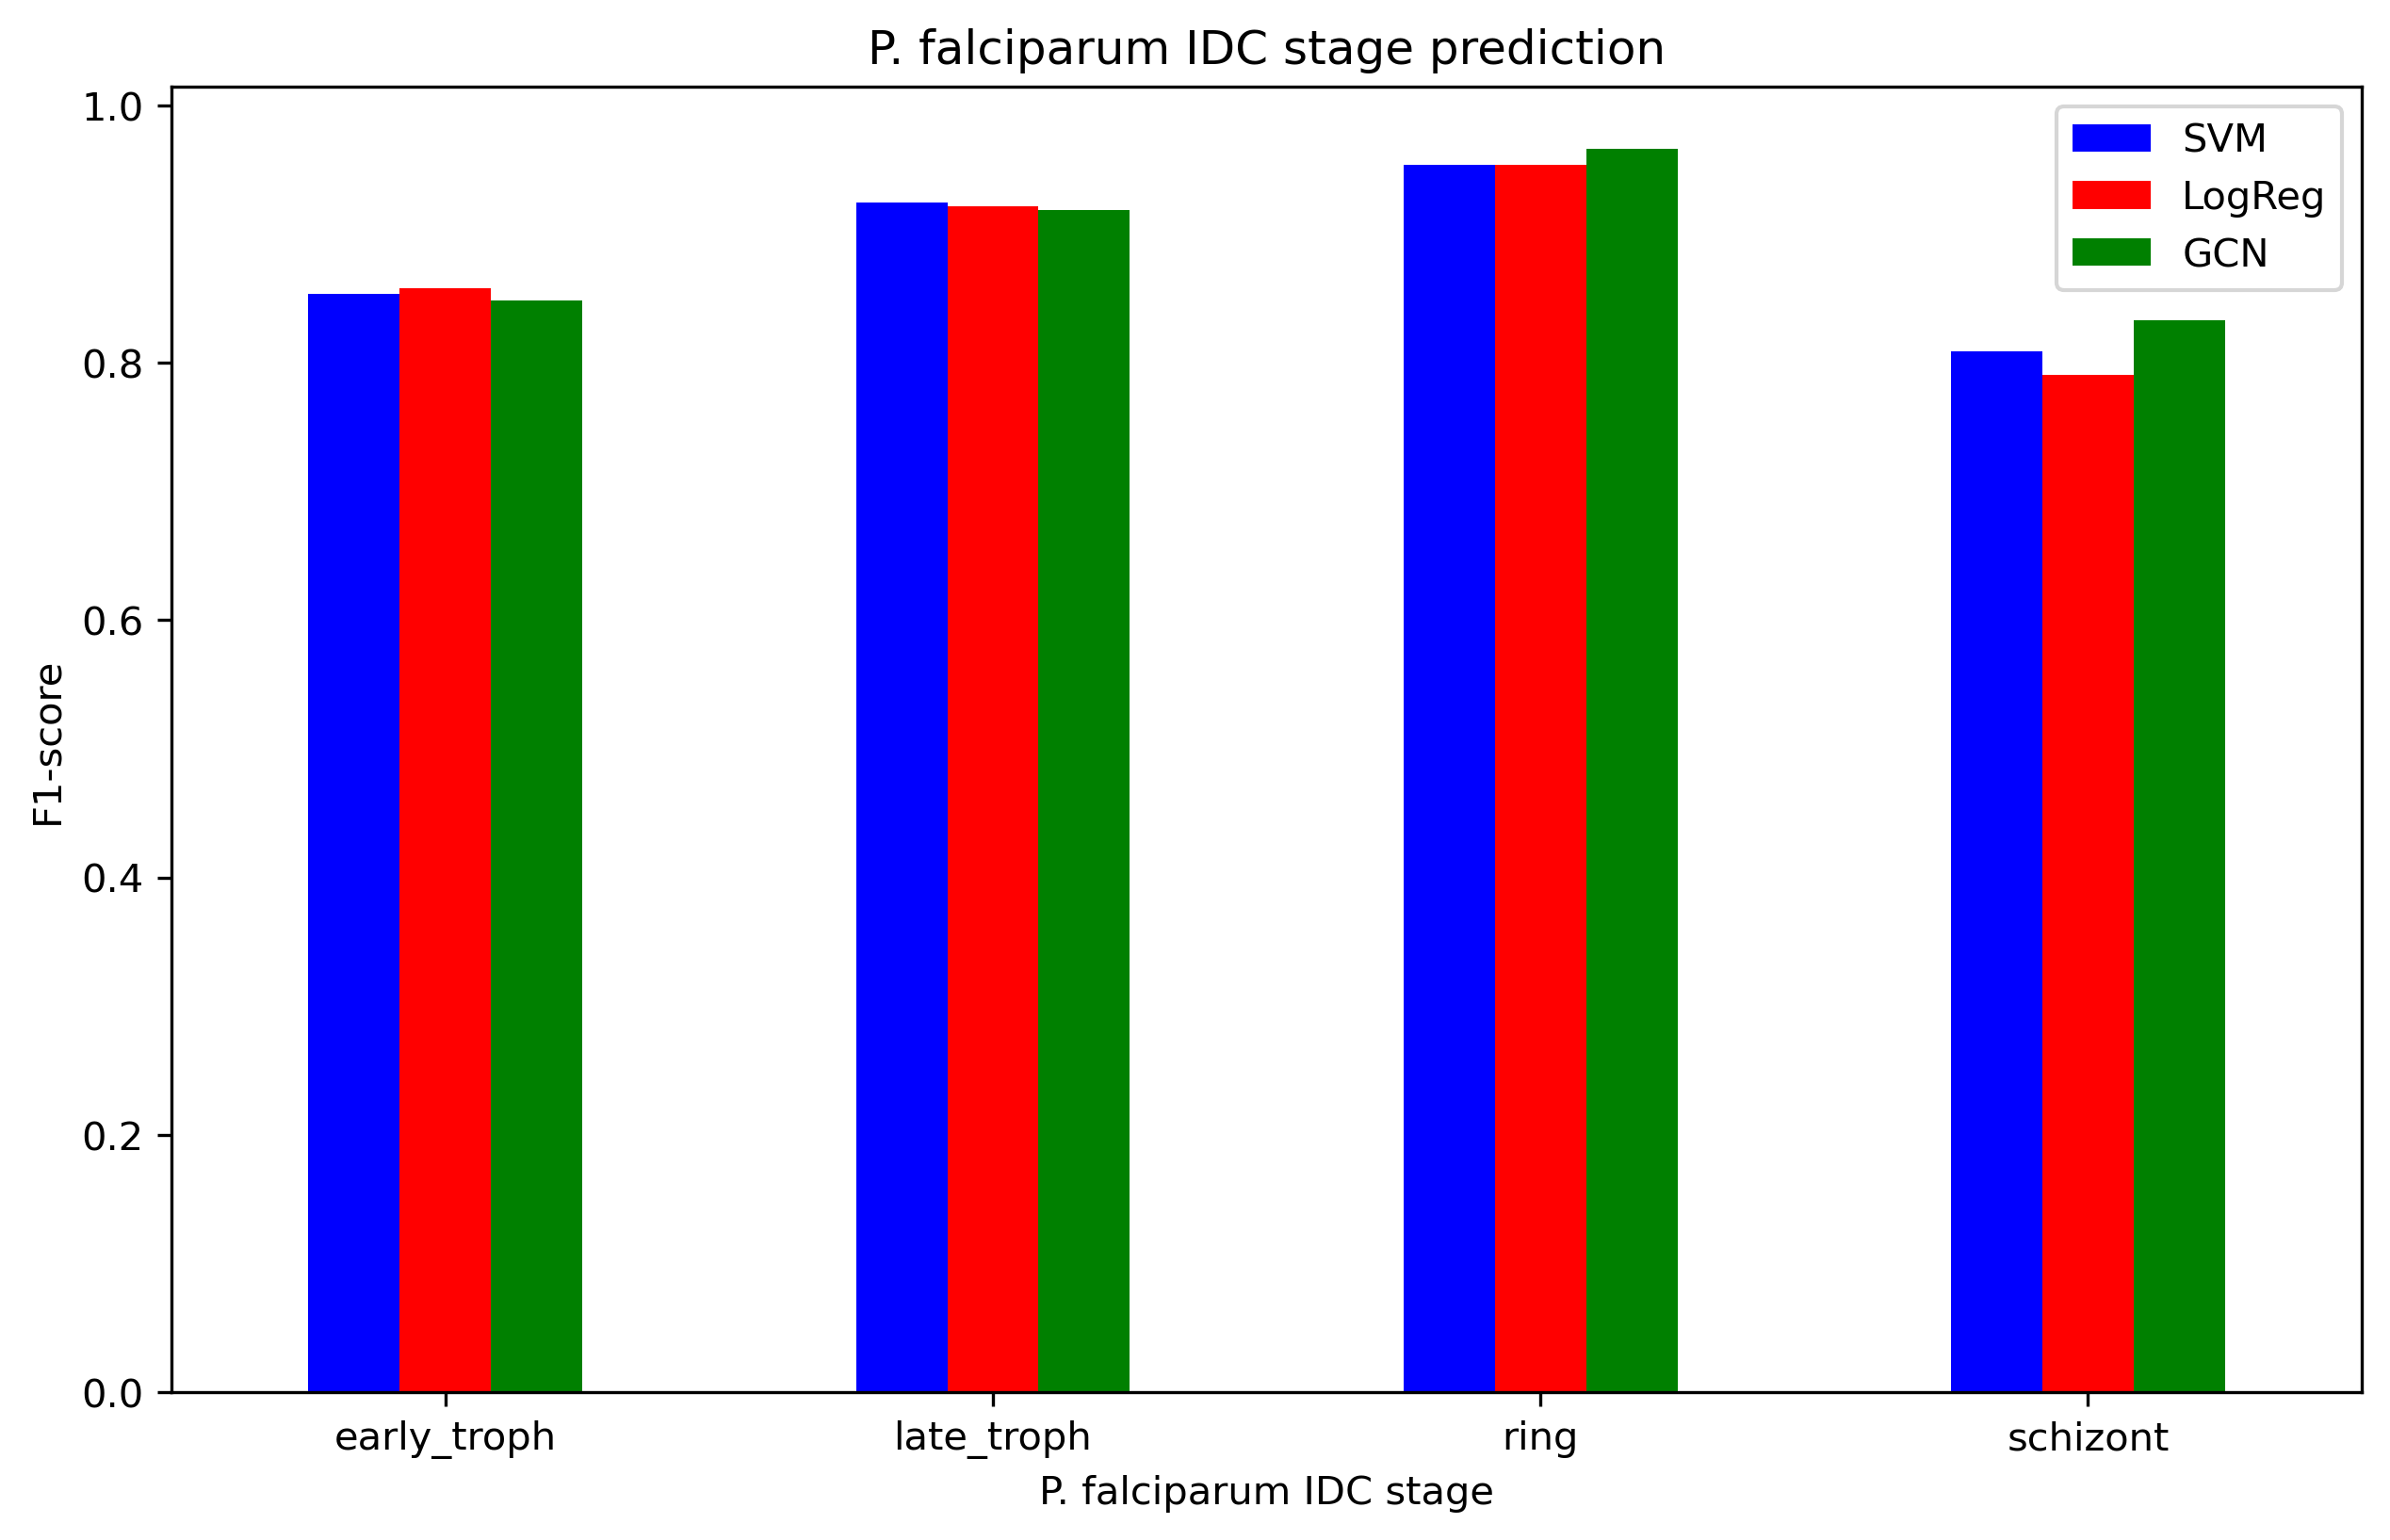
\includegraphics[width=0.8\textwidth]{figures/Pf_prediction.png}
  \caption{Prediction accuracy of models on \textit{P. falciparum} single cell RNA sequencing data.}
	\label{fig:pfal_pred_f1}
\end{figure}

\subsection{Additional Datasets}

We collated a list of scRNAseq datasets, which represent non-human, non-mouse datasets from a wide array of organisms and reference human and mouse datasets (Table \ref{tab:dat_summary}). The organisms include malaria, parasitic worm \emph{Schistosoma mansoni}, the cause of African sleeping sickness \emph{Trypanosoma brucei}, tick borne parasite \emph{Babesia microti}, zebrafish, and non-human primates. Through training and testing our model on a variety of organisms, we hope to create a model that transcends the need for manual knowledge and can find biomarkers of different cell types to better characterize these diseases. 

\begin{table}[!h]
  \caption{Summary of datasets that will be used in this study.}
  \label{tab:dat_summary}
  \centering
  \begin{tabularx}{\textwidth}{lXll}
    \toprule
    \textbf{Host} & \textbf{Source} & \textbf{Reference} & \textbf{Cells} \\
    \midrule
    Parasite & \href{https://github.com/vhowick/MalariaCellAtlas/tree/4e19a713d0681b118cc7e229133489f039b8766b/Expression_Matrices/10X/pf10xIDC}{GitHub} & \citet{howickMalariaCellAtlas2019} & 6,737 \\
    \midrule
    Parasite & \href{https://www.ncbi.nlm.nih.gov/geo/query/acc.cgi?acc=GSE146737}{GEO: GSE146737} & \citet{wendtSinglecellRNAseqAtlas2020} & 43,642 \\
    \midrule
    Parasite & \href{https://zenodo.org/records/5163554}{Zenodo: 5163554} & \citet{briggsSinglecellTranscriptomicAnalysis2021} & 8,599 \\
    \midrule
    Parasite & \href{https://github.com/umbibio/scBabesiaAtlases}{Github} & \citet{rezvaniComparativeSinglecellTranscriptional2022} & 8,719-12,910 \\
    \midrule
Human & \href{https://doi.org/doi:10.18129/B9.bioc.TENxPBMCData}{TENxPBMCData R Package} & \citet{hansenTENxPBMCData2018} & 3,000 \\
    \midrule
    Human & \href{https://doi.org/doi:10.18129/B9.bioc.scRNAseq}{scRNAseq R Package
} & \citet{rissoScRNAseq2017, lawlorSinglecellTranscriptomesIdentify2017} & 978 \\
    \midrule
    Human & \href{https://www.ncbi.nlm.nih.gov/geo/query/acc.cgi?acc=GSE151530}{GEO: GSE151530} & \citet{maMultiregionalSinglecellDissection2022} & 56,721 \\
    \midrule
    Mouse & \href{https://doi.org/doi:10.18129/B9.bioc.scRNAseq}{scRNAseq R Package} & \citet{rissoScRNAseq2017, zeiselCellTypesMouse2015} & 3,005 \\
    \midrule
    Zebrafish & \href{https://www.ncbi.nlm.nih.gov/geo/query/acc.cgi?acc=GSE106587}{GEO: GSE106587} & \citet{farrellSinglecellReconstructionDevelopmental2018}  & 38,731 \\
    \midrule
    Non-human primate & \href{https://www.ncbi.nlm.nih.gov/geo/query/acc.cgi?acc=GSE156755}{GEO: GSE156755} & \citet{speranzaSinglecellRNASequencing2021} & 100,795 \\
    \bottomrule
  \end{tabularx}
\end{table}

\section{Future Plans}

\subsection{Continued Data Curation}

The datasets represented in Table 1 have to be accessed from their data repositories to obtain the cell x gene matrix, which will undergo quality control filtering and normalization. 


\subsection{Cross Validation}
Rather than simple test/train splits, we will implement cross-validation across all tested models. 


\subsection{Transformer Model}

We are working on implementing a minimal single head attention network using Pytorch \cite{paszkePyTorchImperativeStyle2019}, based on the defining paper Attention is All you Need \cite{vaswaniAttentionAllYou2023}. Yet there are several challenges we must address in order to generalize ‘standard’ models for use with gene expression data. First, gene expression, as currently measured, is inherently unordered, i.e. there is no need for positional encoding of each token (gene). Therefore it would be ideal to not limit the input sequence length so global gene-gene interactions can be captured. However, the memory and time complexity scale quadratically  with input length, which limits standard models to an input length of around 500 in practice. There have been several publications, including Reformer and Performer, that each aimed to improve transformer efficiency \cite{katharopoulosTransformersAreRNNs2020, daiTransformerXLAttentiveLanguage2019, meritySingleHeadedAttention2019, choromanskiRethinkingAttentionPerformers2022, kitaevReformerEfficientTransformer2020, vyasFastTransformersClustered2020}. We are working to adapt the Performer method to our simpler model. 

In the human and mouse datasets that can be input into scBERT and TOSICA, we will implement these methods and classical methods, such as logistic regression, random forest and support vector machines, to compare the classification accuracy of our method. 

\subsection{Reproducibility}

Although there is a growing awareness of the 'reproducibility  crisis' in research, many computational biological studies continue to only make part of their code and analysis publicly available. We are striving to proactively organize our analysis in an open and easy-to-reproduce structure. This includes, but is not limited to, using: pinned dependency and dataset versions, Docker, Git, and Make/Snakemake. Our final analysis will be available at: https://github.com/RyanVidegar-Laird/gettention (bad name subject to change).


\subsection{Division of Work}
We will split the preparation of the remaining 9 datasets in thirds, where Sean will prepare the three parasite datasets, Ryan will prepare the three human datasets and Stephanie will prepare the mouse, zebrafish, and other non-human primate datasets.

For the final report, Stephanie will expand on the introduction and related work. Ryan will write up the methods and some of the results. Sean will help write up the results and conclusion. We will all contribute to editing the final report.


\bibliography{final_report}

\end{document}